In this section we discuss the algorithms evaluated in our two online
trials\footnote{All code used in these experiments is available at
\url{http://code.google.com/p/social-recommendation/}.  The conditions
of our ethics approval \#2011/142 from the Australian National
University for conducting human trials on Facebook require our
privacy policy
(\url{http://dmm.anu.edu.au/linkr/website/pp.php}) to
prohibit public sharing of data collected during these experiments.}
and additional analysis regarding trends and patterns in our social
recommendation setting.

\subsection{First Trial}

In our first trial, our objective was to evaluate four CF and SCF
approaches to establish which was the most promising direction for
SCF extension:
\begin{enumerate}
\item {\bf $k$-Nearest Neighbor (KNN)}: See Section~\ref{sec:nn}.
\item {\bf Support Vector Machines (SVM)}: See Section~\ref{sec:cbf}.
\item {\bf Matchbox (Mbox)}: simple Matchbox CF %Optimization of the $L_2$ regularized Matchbox objective:
$$\Obj_\pmcf + \lambda \Obj_\ru + \lambda \Obj_\rv$$
\item {\bf Social Matchbox (Soc. Mbox)}: %Optimization of the 
%$L_2$ and 
feature-based \emph{socially regularized} Matchbox SCF
$$\Obj_\pmcf + \lambda_\rs \Obj_\rs + \lambda \Obj_\ru + \lambda \Obj_\rv$$
\end{enumerate}
KNN and MBox may be viewed as pure CF methods.  As discussed previously,
both SVM and Soc. Mbox may be viewed as SCF methods; all objectives
for these were given in Section~\ref{sec:NewObjFuns}
and were both optimized via gradient descent as outlined
in Appendix~\ref{app:Derivatives}.  

The first live user trial was run from August 25, 2011 to October 13, 2011 
with 108 users and yielded 2,493 combined like and 
dislike ratings of recommended
links over the 49 day period.  Algorithms were assigned randomly to the
users with assignment counts shown in Table~\ref{tab:Assigned1} (left).

%%%%%%%%%%%%%%%%%%%%%%%%%%%%%%%%%%%%%%%%%%%%%%%%%%%%%%%%%%
\begin{table}[t!]
\centering
\begin{minipage}{1.5in}
\begin{tabular}{| l | c |}
\hline
{\bf Algorithm} & {\bf Users} \\
\hline
Soc. Mbox & 26\\
Mbox  & 26 \\
SVM & 28 \\
KNN & 28 \\
\hline
\end{tabular}
  \end{minipage}
  \begin{minipage}{1.3in}
\begin{tabular}{| l | c |}
\hline
{\bf Algorithm} & {\bf Users} \\
\hline
Soc. Mbox & 26\\
Spec. Mbox  & 25 \\
Spec. CP & 27 \\
Soc. Hybrid & 25 \\
\hline
\end{tabular}
  \end{minipage}
\caption{Number of users assigned per algorithm in the first trial (left)
and second trial (right).}
\label{tab:Assigned1}
\end{table}
%%%%%%%%%%%%%%%%%%%%%%%%%%%%%%%%%%%%%%%%%%%%%%%%%%%%%%%%%%

As shown in Figure~\ref{fig:OnlineResult1}, Soc. Mbox was the
best performing algorithm in the first trial and in fact was the only
algorithm to receive more like ratings than dislike ratings. 
This suggests that using social regularization in conjunction with
MF-based CF does indeed provide more useful information than simple
MBox without social regularization.  We also note a
significant drop in performance between recommending friend links and
recommending non-friend links, indicating that users had a bias to
like links recommended by friends more (importantly, we note that
users could see the names and comments of friends whose links were recommended).
%%%%%%%%%%%%%%%%%%%%%%%%%%%%%%%%%%%%%%%%%%%%%%%%%%%%%%%%%%
\begin{figure*}[t!]
\centering
\subfigure{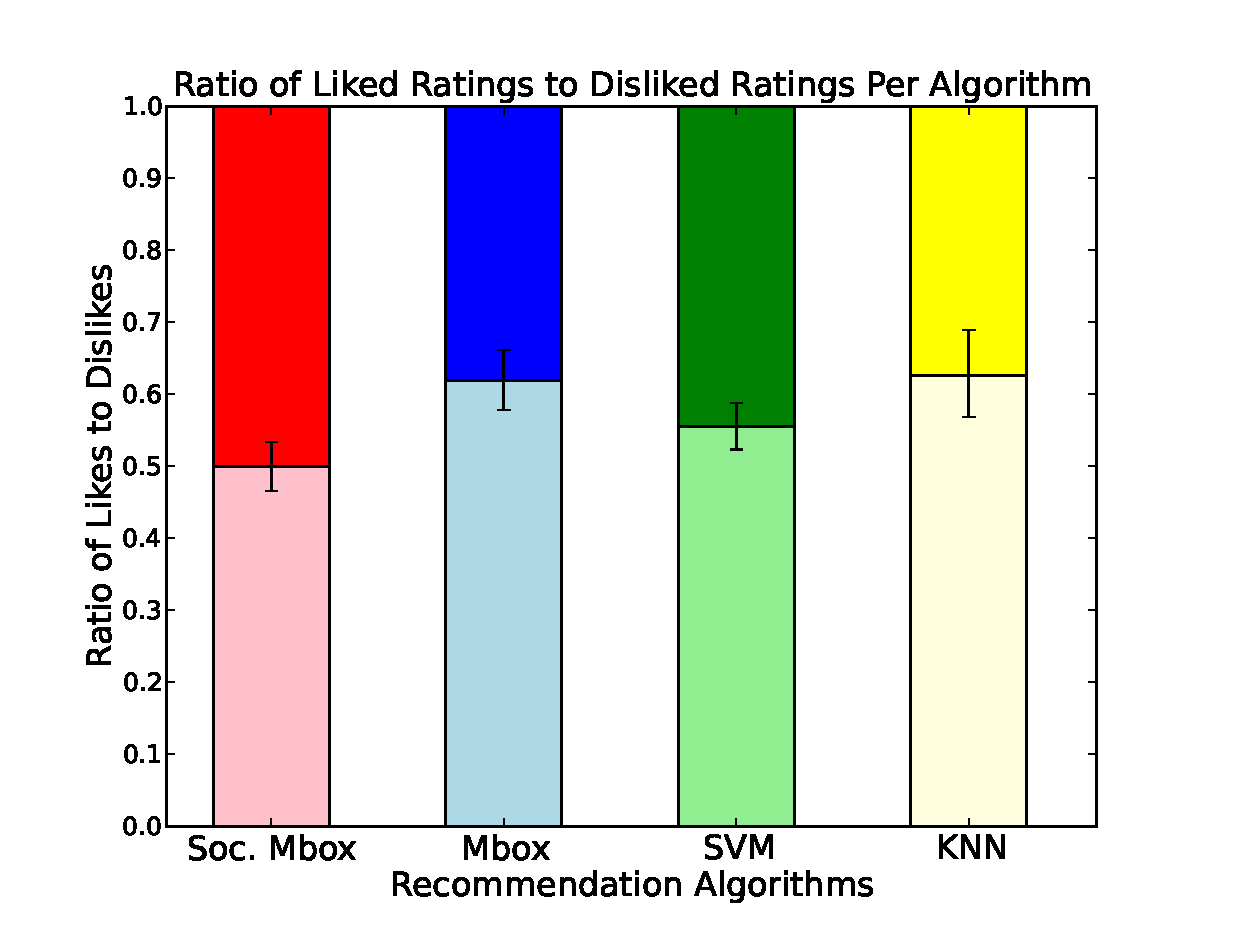
\includegraphics[scale=0.28]{img_new/live-likes1-orig.eps}}
\subfigure{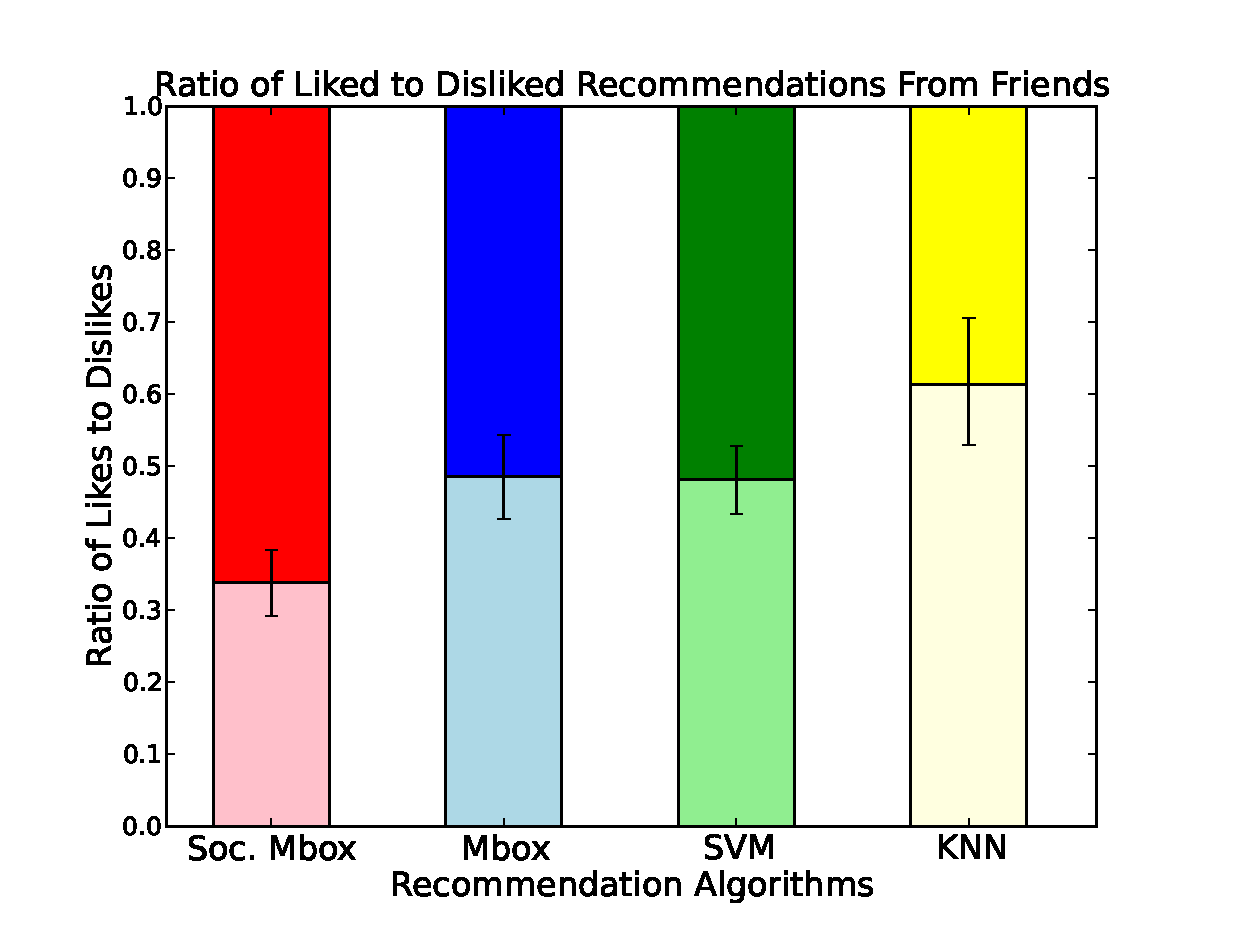
\includegraphics[scale=0.28]{img_new/live-friend-likes1-orig.eps}}
\subfigure{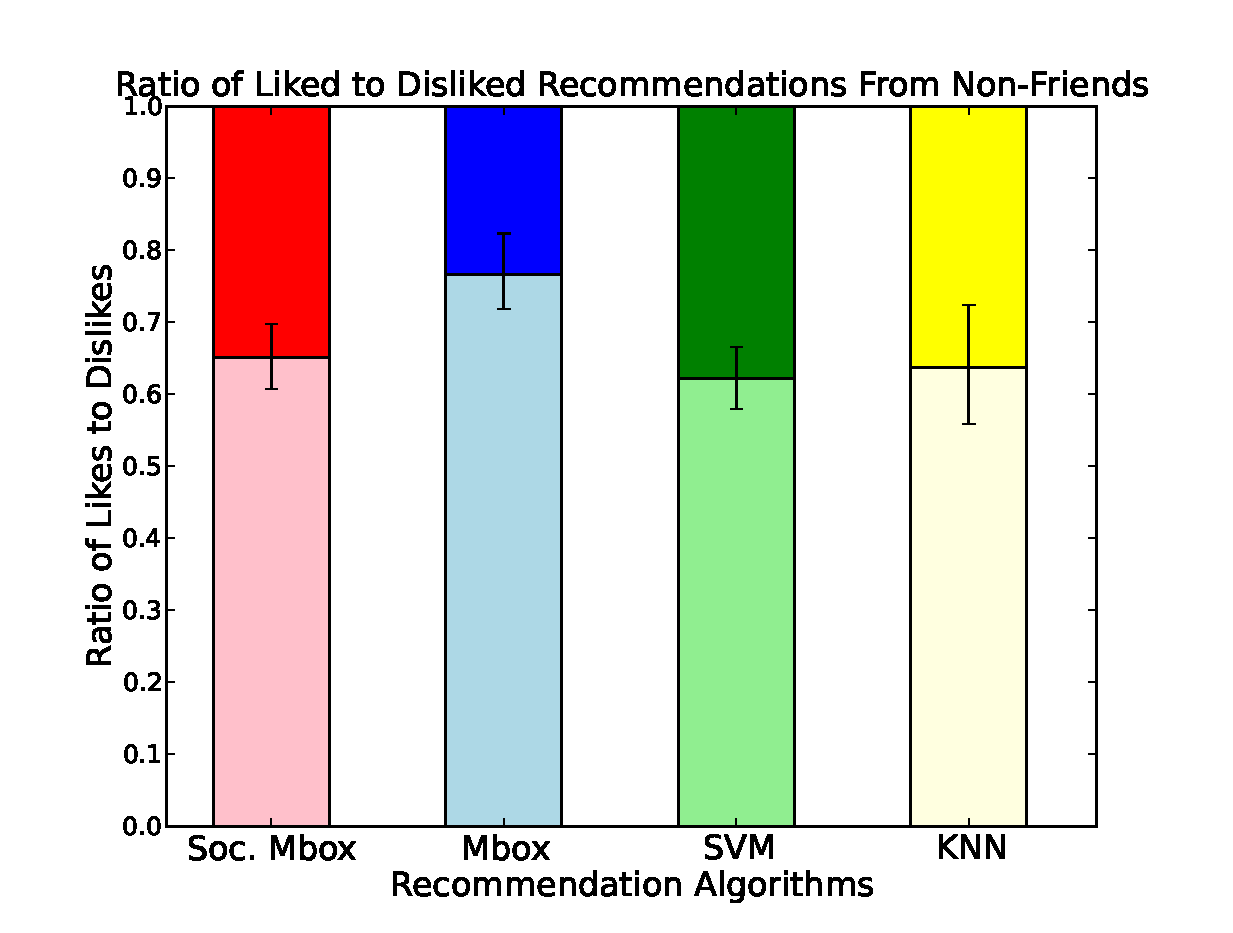
\includegraphics[scale=0.28]{img_new/live-nonfriend-likes1-orig.eps}}
\caption{Stacked bar graphs of online results for the first 
user trial.  The fraction of likes is displayed above 
the fraction of dislikes.  (left) all links, (center) friend links,
(right) non-friend links.  The 95\% confidence interval on all 
results is $< \pm 0.02$ so all differences are signficant
except for MBox and SVM in the center and the virtual tie
between three algorithms on the right.}
\label{fig:OnlineResult1}
\end{figure*}
%%%%%%%%%%%%%%%%%%%%%%%%%%%%%%%%%%%%%%%%%%%%%%%%%%%%%%%%%%

%%%%%%%%%%%%%%%%%%%%%%%%%%%%%%%%%%%%%%%%%%%%%%%%%%%%%%%%%%
%%%%%%%%%%%%%%%%%%%%%%%%%%%%%%%%%%%%%%%%%%%%%%%%%%%%%%%%%%

\subsection{Second Trial} 

For the second online trial, we again chose four algorithms to
randomly assign to the LinkR application users.  Social Matchbox
was included again as a baseline since it was the best performing
algorithm in the first trial.  The remaining three algorithms
were all relatively orthogonal extensions (or variants) of Social Matchbox
based on the \emph{three novel objective functions} defined in 
Section~\ref{sec:newobjfun_defs}:
\begin{itemize}
\item {\bf Social Matchbox (Soc. Mbox)} : unchanged.
\item {\bf Spectral Matchbox (Spec. Mbox)}: 
$$\Obj_\pmcf + \lambda_\rss \Obj_\rss + \lambda \Obj_\ru + \lambda \Obj_\rv$$
%Matchbox MF + Social Spectral Regularization + L2 $U$ Regularization + L2 $V$ Regularization
\item {\bf Social Hybrid (Soc. Hybrid)}: 
$$\lambda_\phy \Obj_\phy + \lambda_\rs \Obj_\rs + \lambda \Obj_\ru + \lambda \Obj_\rv + \lambda \Obj_\rw$$
%Hybrid + Social Regularization + L2 $U$ Regularization + L2 $V$ Regularization + L2 $\w$ Regularization
\item {\bf Spectral Co-preference (Spec. CP)}: 
$$\Obj_\pmcf + \lambda_\rscs \Obj_\rscs + \lambda \Obj_\ru + \lambda \Obj_\rv$$
%Matchbox MF + Social Co-preference Spectral Regularization + L2 $U$ Regularization + L2 $V$ Regularization
\end{itemize}
All objectives are defined in Section~\ref{sec:NewObjFuns} 
and optimized via gradient descent as outlined
in Appendix~\ref{app:Derivatives}.  

The second trial with the above algorithms ran from October 13, 2011
to November 5, 2011 with 103 users and yielded 1,435 like/dislike
ratings of recommended links over the 24 day period; on the start of
the second trial, users were notified that they would be randomly
assigned to new algorithms and encouraged to re-engage with the LinkR
App if they had not been using it.  The distribution of the algorithms
to the users is shown in Table~\ref{tab:Assigned1} (right).

%%%%%%%%%%%%%%%%%%%%%%%%%%%%%%%%%%%%%%%%%%%%%%%%%%%%%%%%%%%%%%%%%%%%%%%%%
\begin{figure*}[t!]
\centering
\subfigure{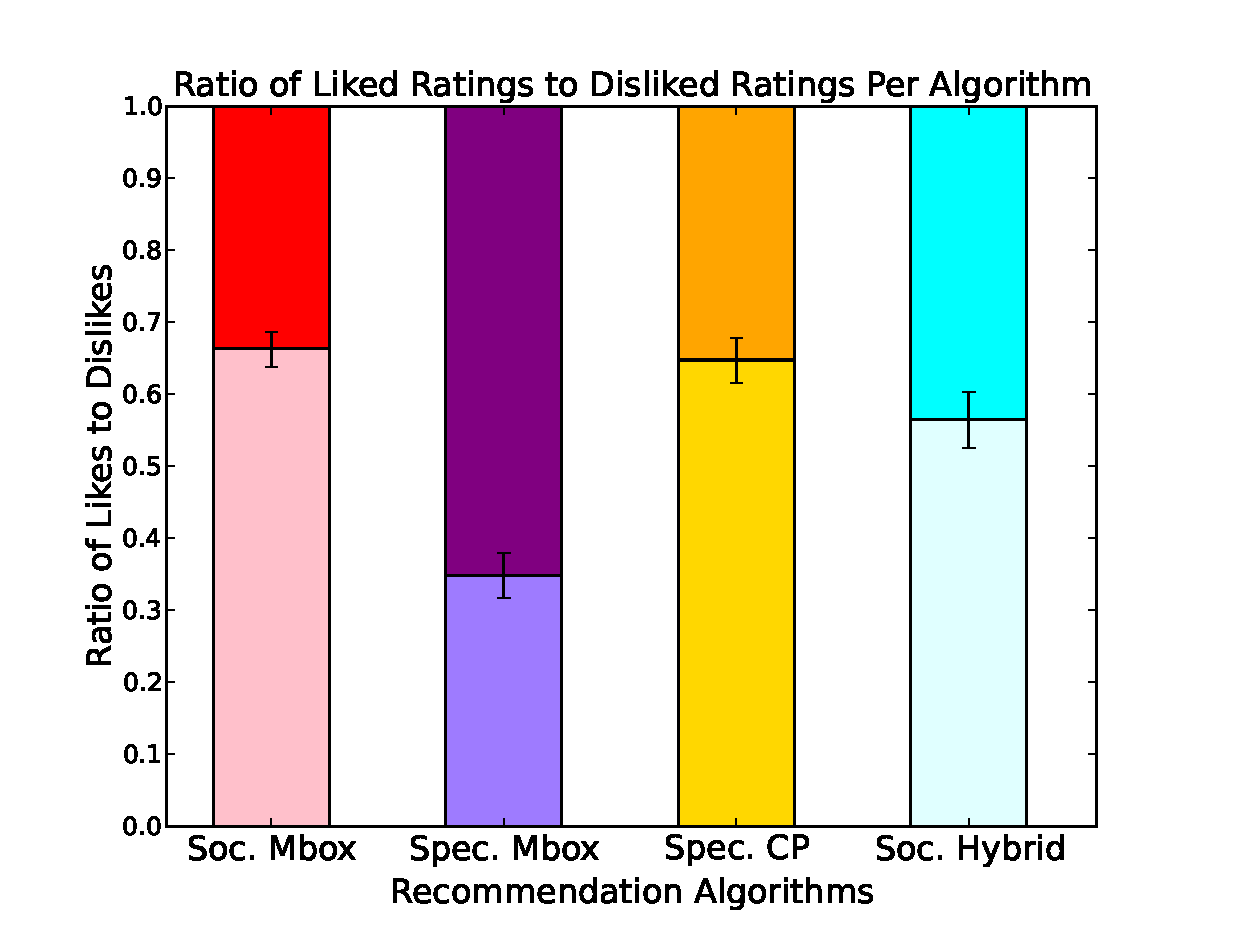
\includegraphics[scale=0.28]{img_new/live-likes2-Feb10.eps}}
\subfigure{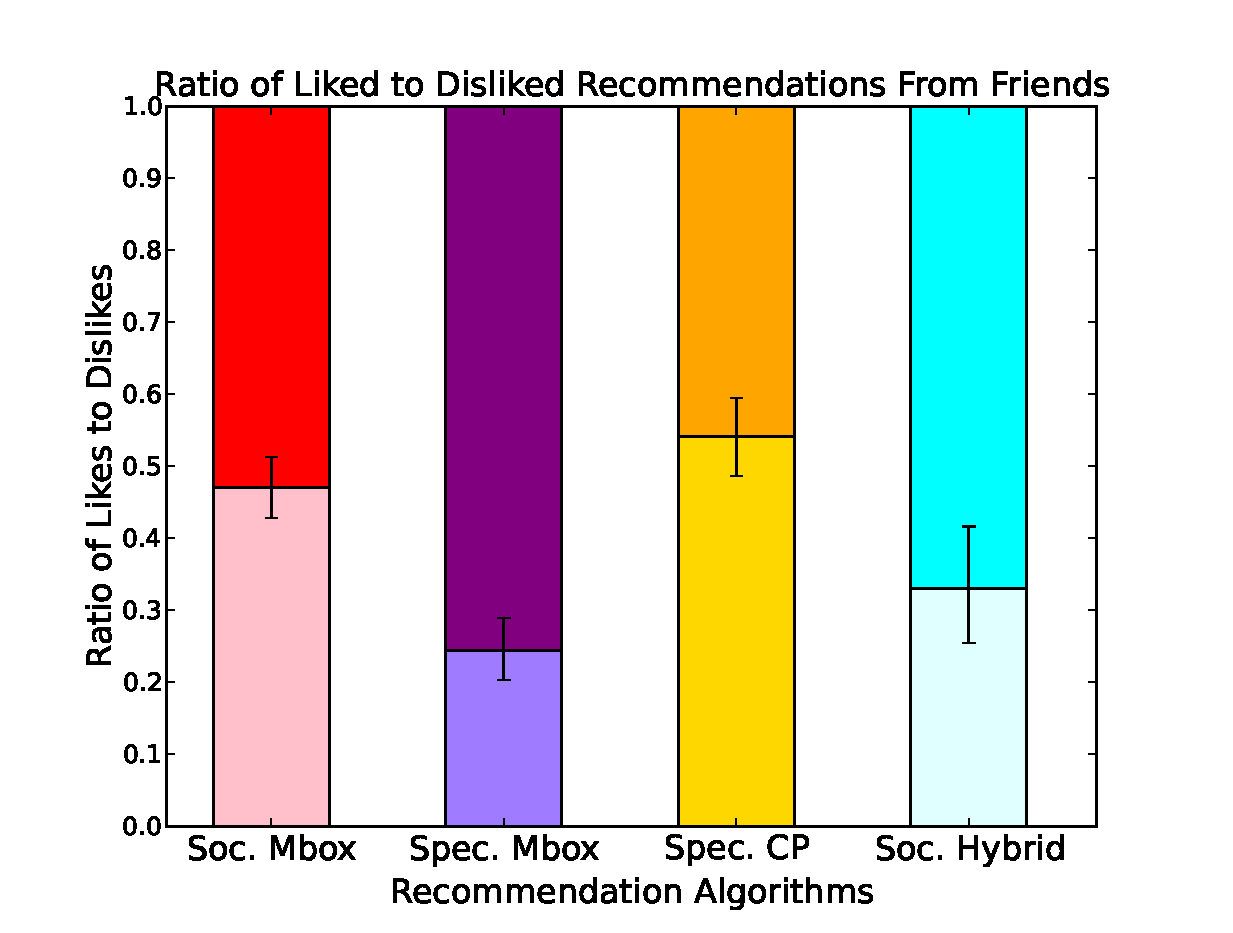
\includegraphics[scale=0.28]{img_new/live-friend-likes2-Feb10.eps}}
\subfigure{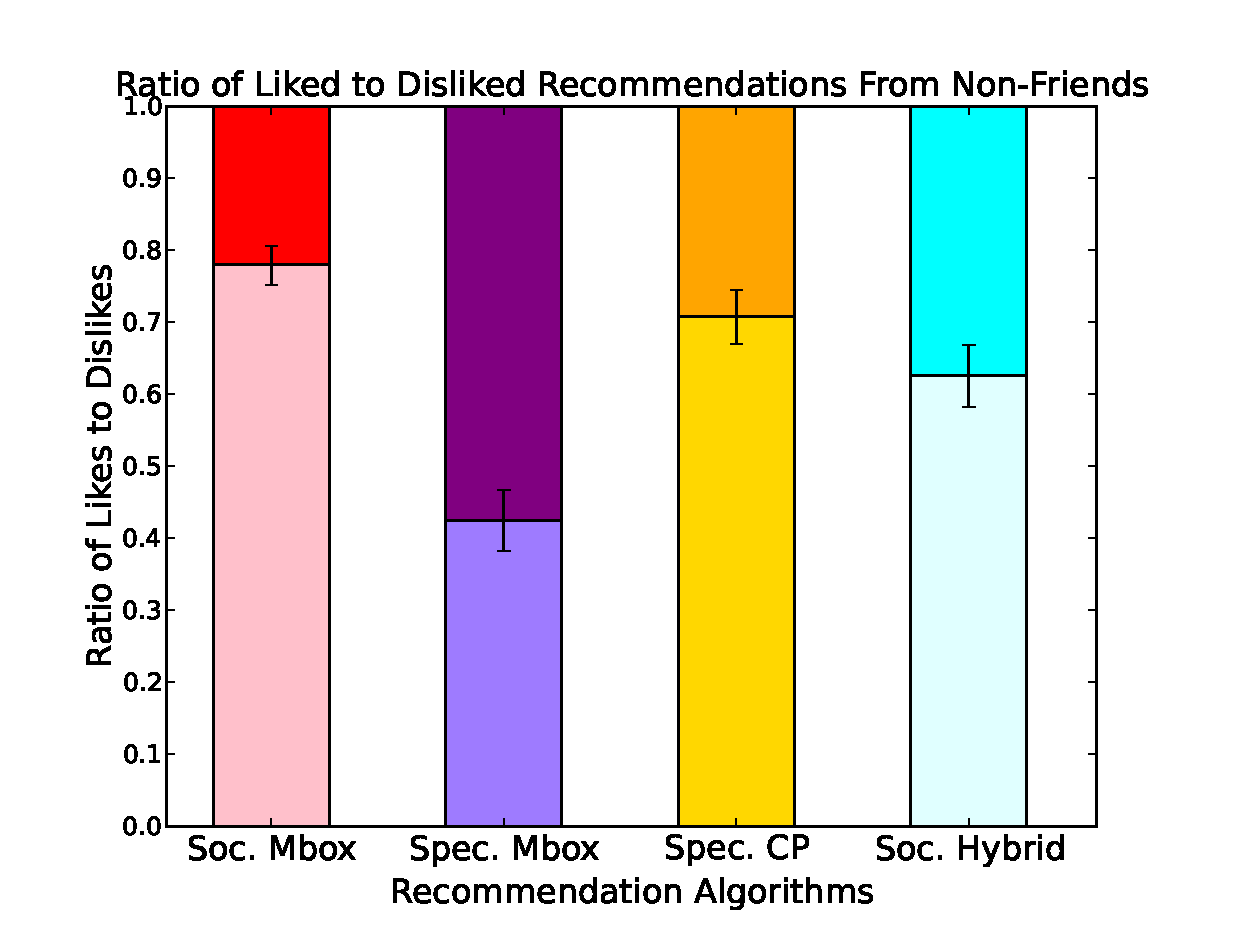
\includegraphics[scale=0.28]{img_new/live-nonfriend-likes2-Feb10.eps}}
\caption{Stacked bar graphs of online results for the second
user trial.  The fraction of likes is displayed above 
the fraction of dislikes.  (left) all links, (center) friend links,
(right) non-friend links. The 95\% confidence interval on all 
results is $< \pm 0.026$ so all differences except Spec. Mbox
and Soc. Hybrid in the center graph are significant. }
\label{fig:online2}
\end{figure*}
%%%%%%%%%%%%%%%%%%%%%%%%%%%%%%%%%%%%%%%%%%%%%%%%%%%%%%%%%%%%%%%%%%%%%%%%%

Results for the second trial are 
shown in Figure~\ref{fig:online2}, following are the key observations:
\begin{itemize}
\item Soc. MBox did not perform as well in the second trial as it had
in the first trial.  One key difference in the second trial is that
all of the first trial data was available for training and thus
Soc. MBox may have proved more difficult to optimize given this larger 
quantity of training data.
\item Spec. Mbox clearly performed the best in the second trial 
and this suggests that spectral social 
regularization is likely a better method of regularization 
than the original social regularization variant.
\item Soc. Hybrid does an excellent job of capturing information diffusion
in the social network and hence performs best on recommending friend
links and most poorly on non-friend links (where there is no direct
user-to-user information diffusion).  Soc. Hybrid slightly outperforms
Spec. MBox, but not statistically significantly given the more limited
data in the second trial.  Nonetheless, 
Soc. Hybrid clearly outperforms its Soc. MBox variant that lacks 
information diffusion features.
\item Spec. CP leads to a statistically significant improvement
on recommending non-friend links over Soc. MBox and Soc. Hybrid,
which perform poorly on recommending non-friend links.  Clearly then
Spec. CP is benefitting somewhat in learning from copreferences
since it can socially regularize across two users that are \emph{not}
friends, unlike the other approaches.
\end{itemize}

%%%%%%%%%%%%%%%%%%%%%%%%%%%%%%%%%%%%%%%%%%%%%%%%%%%%%%%%%%
%%%%%%%%%%%%%%%%%%%%%%%%%%%%%%%%%%%%%%%%%%%%%%%%%%%%%%%%%%

\subsection{User Behavior Analysis}

\label{sec:behavior}

Here we briefly analyze user behavior during both trials of the Facebook
LinkR App that can be helpful in building future SCF systems.

\subsubsection{Click evidence}

In Figure~\ref{fig:click_evidence}, we observe the ratings of links
that users clicked on.  The most important thing we notice in 
Figure~\ref{fig:click_evidence} (left) is that even though users
clicked on a link, they were somewhat likely to rate it as a dislike.

One might hypothesize that perhaps users clicked on links more often with
no description to find out what they were and most often disliked them ---
this might explain the high number of dislikes for clicked links.  However,
examining both 
Figure~\ref{fig:click_evidence} (center) and (right)
for non-friend links, we observe that whether a description was present
had very little impact on whether a link was liked or not, so we cannot
infer that all the disliked links were simply the ones lacking a description.

Then the insight from this analysis is extremely important 
for SCF recommendation design because it states that click data is a very
weak indicator of likes and explicit feedback should be used if at all
possible.

%%%%%%%%%%%%%%%%%%%%%%%%%%%%%%%%%%%%%%%%%%%%%%%%%%%%%%%%%%
\begin{figure*}[t!]
\centering
\subfigure{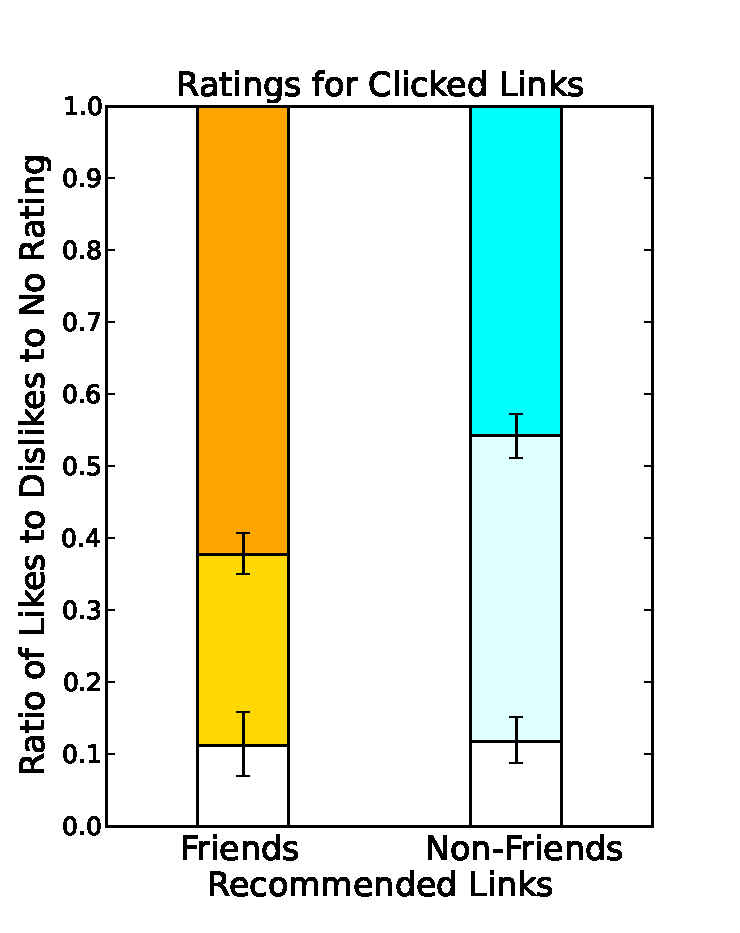
\includegraphics[width=24mm,height=43mm]{img_new/clicked-likes.eps}}
\hspace{-4mm}
\subfigure{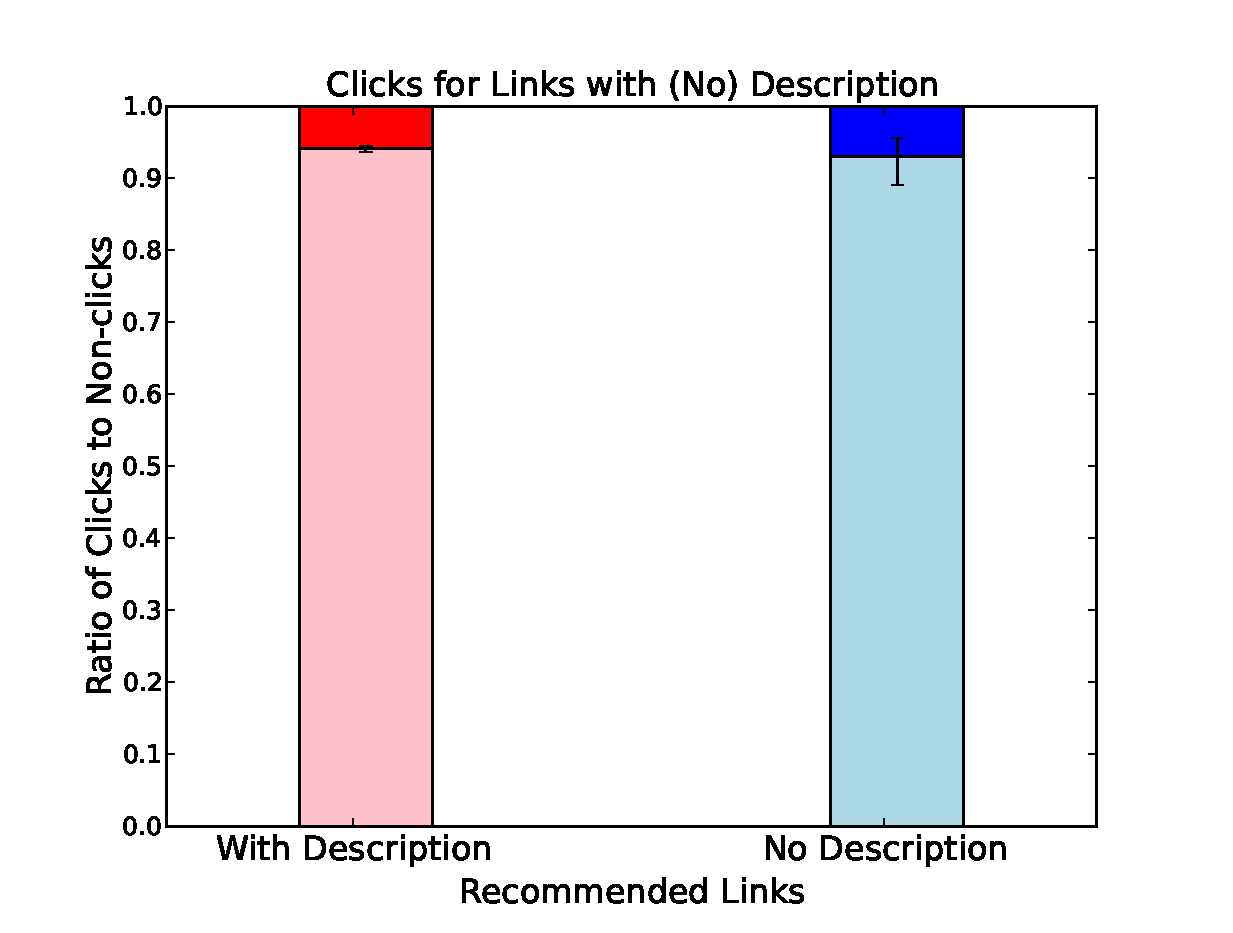
\includegraphics[width=24mm,height=43mm]{img_new/description-clicked.eps}}
\hspace{-4mm}
\subfigure{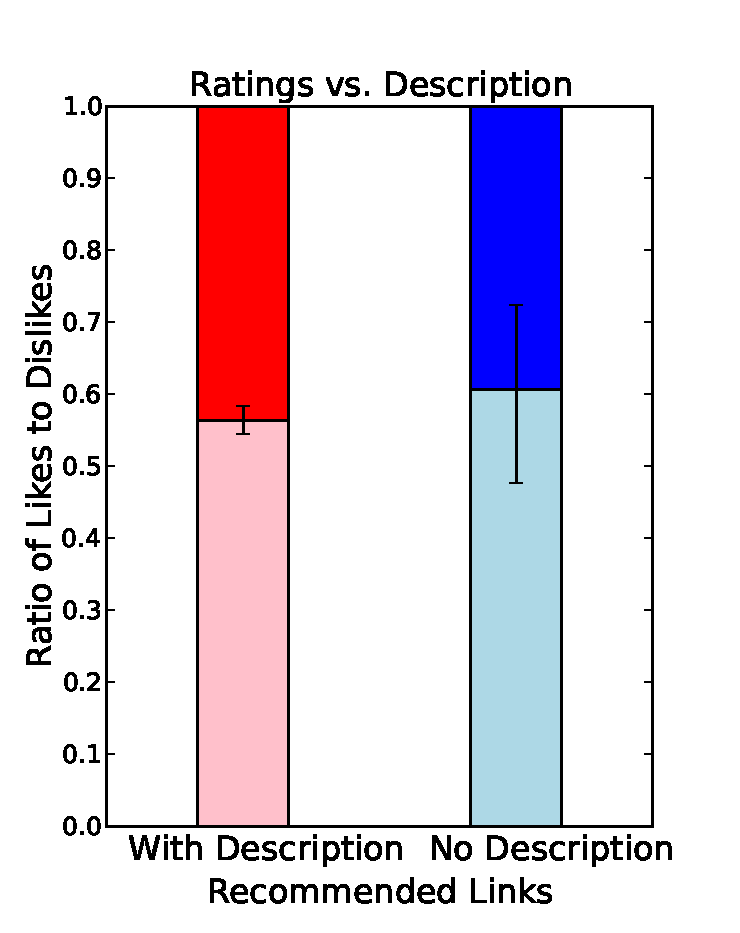
\includegraphics[width=24mm,height=43mm]{img_new/description-liked.eps}}
\hspace{-4mm}
\subfigure{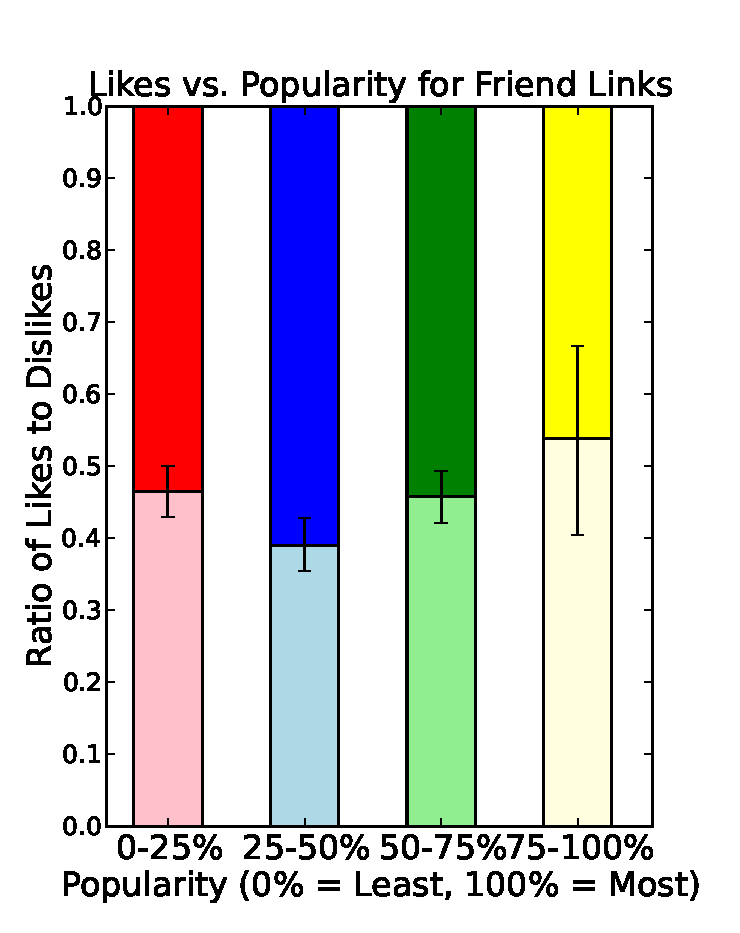
\includegraphics[scale=0.28]{img_new/friend-popularity.eps}}
\hspace{-6mm}
\subfigure{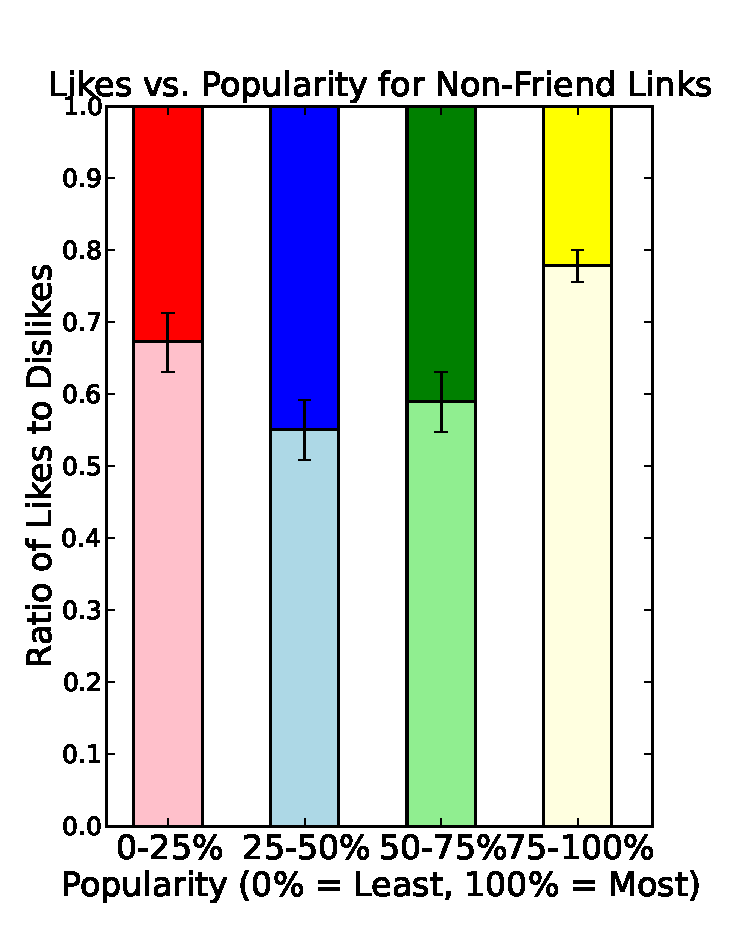
\includegraphics[scale=0.28]{img_new/non-friend-popularity.eps}}
\caption{Stacked bar graphs of online results for the first 
user trial.  The fraction of likes (or clicks) is displayed above 
the fraction of dislikes (or non-clicks) -- and above the fraction of not-rated
links for the left-most figure.  
(left) ratings for clicked links, (center) click rates if
text description not present, 
(right) percentage liked if click description not present.
Stacked bar graphs of online results for the first 
user trial.  The fraction of likes is displayed above the fraction of
dislikes.  Shown are the ratings vs. quartile of popularity for (left)
friend and (right) non-friend links.
Stacked bar graphs of online results for the first 
user trial.  The fraction of likes is displayed above the fraction of
dislikes.  Shown are the ratings vs. quartile of popularity for (left)
friend and (right) non-friend links.
}
\label{fig:click_evidence}
\end{figure*}
%%%%%%%%%%%%%%%%%%%%%%%%%%%%%%%%%%%%%%%%%%%%%%%%%%%%%%%%%%

\subsubsection{Impact of Popularity}

In Figure~\ref{fig:popularity} we analyze the impact of global link
popularity (in terms of total shares on Facebook) 
on how much Facebook LinkR App users liked a link.
The trend is clear for both friend (left) and non-friend (right)
links: users tend to like the most popular (top quartile) 
links the least, or at least as much as the least popular (bottom quartile)
links.  In general users tended to prefer links that were somewhat
popular (second highest quartile).  From this we can infer that
link popularity should not be used too heavily in determining link
recommendations since clearly the most popular links are not liked
the most on average.

%%%%%%%%%%%%%%%%%%%%%%%%%%%%%%%%%%%%%%%%%%%%%%%%%%%%%%%%%%
\begin{figure*}[t!]
\centering
%\subfigure{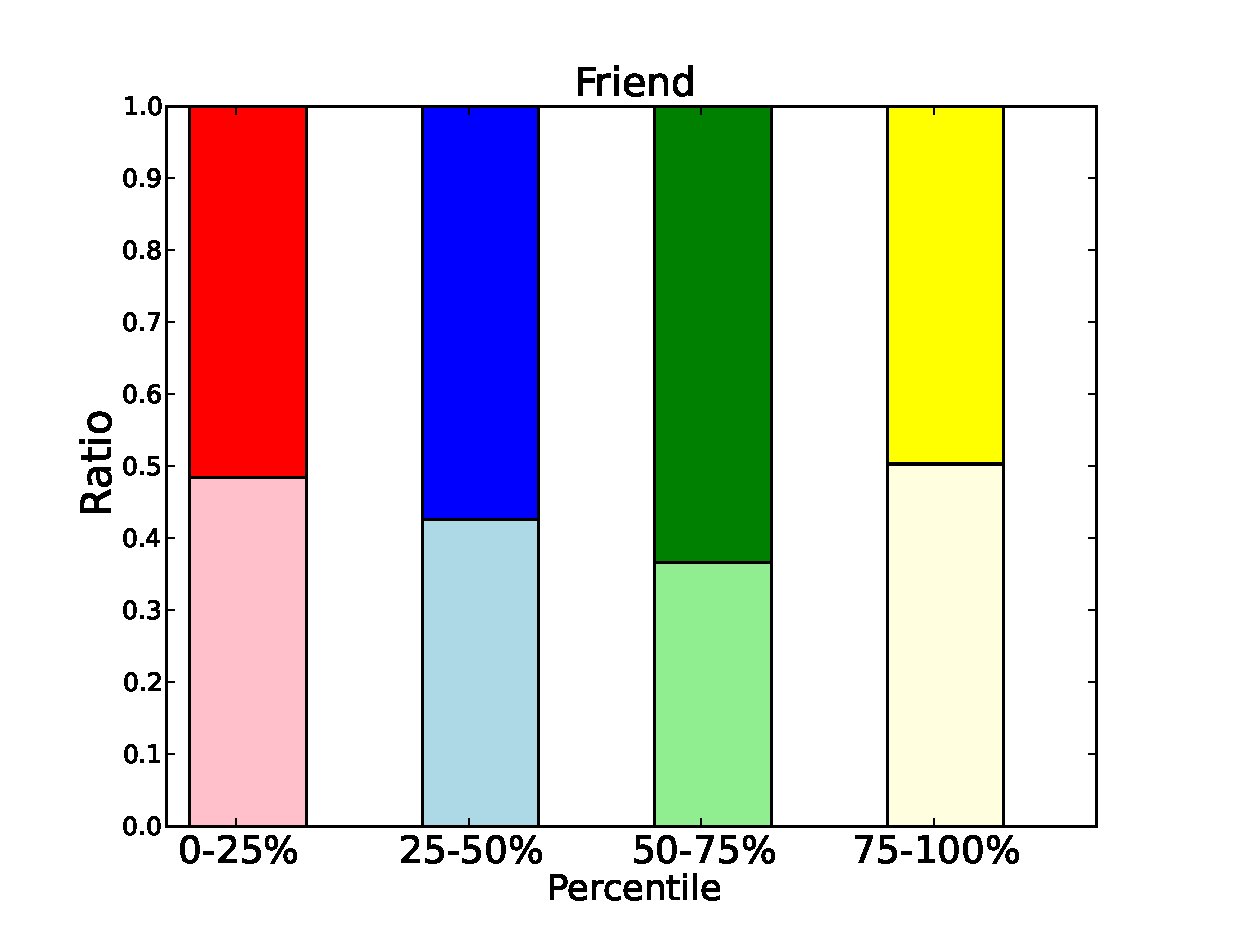
\includegraphics[scale=0.28]{img/percentileFriend.eps}}
%\subfigure{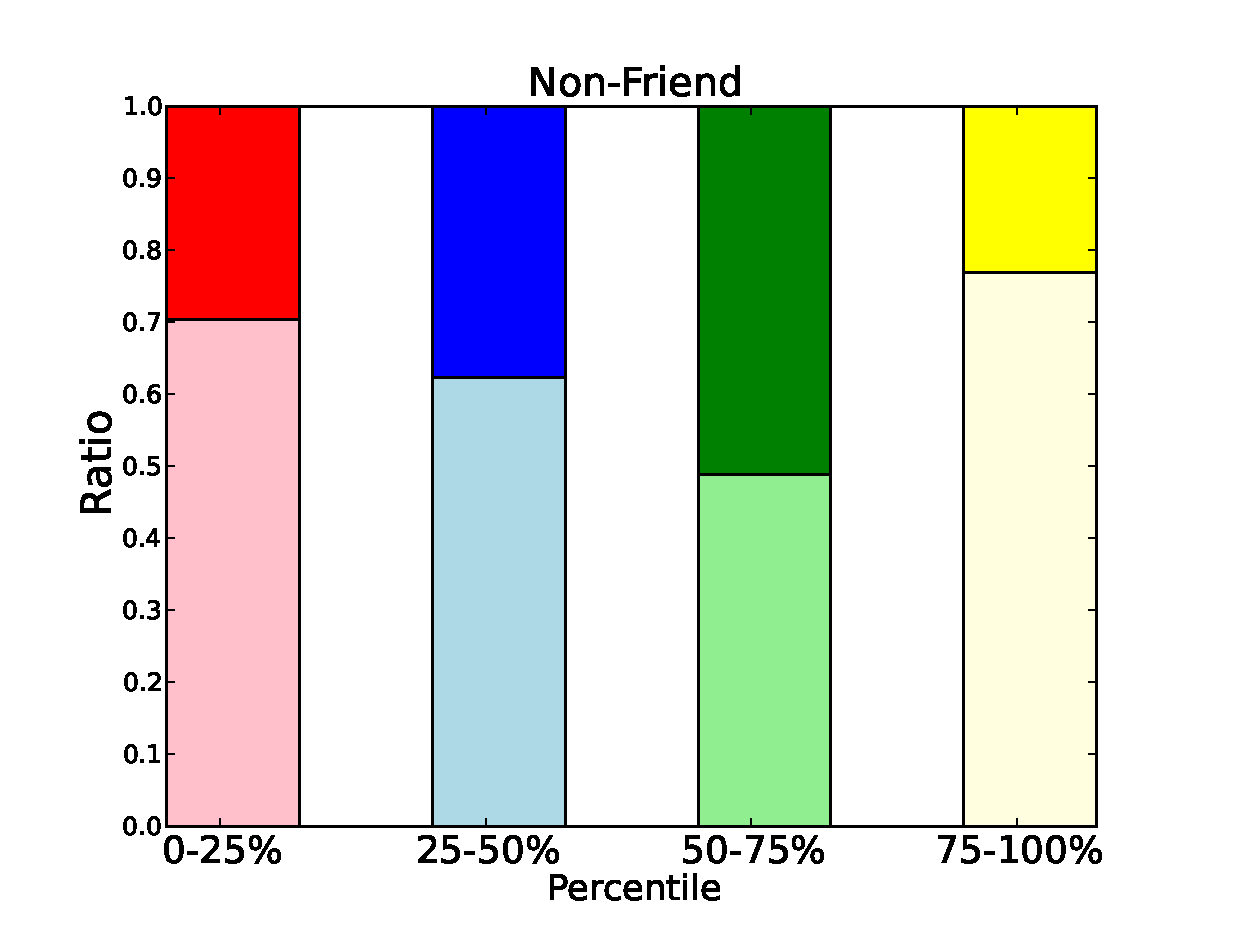
\includegraphics[scale=0.28]{img/percentileNon-Friend.eps}}
\caption{***}
\label{fig:popularity}
\end{figure*}
%%%%%%%%%%%%%%%%%%%%%%%%%%%%%%%%%%%%%%%%%%%%%%%%%%%%%%%%%%

